\documentclass[]{article}

\usepackage[utf8]{inputenc}
\usepackage[portuguese]{babel}
\usepackage{graphicx}
\usepackage{xspace}
\usepackage[font={small, it}]{caption}

\newcommand{\figref}[1]{figura \ref{#1}}

%opening

\title{Ferramenta IPMT}
\author{Jamerson Lima - jfpl@cin.ufpe.br \and Márcio Barbosa - mbof@cin.ufpe.br}
\date{}

\begin{document}

\maketitle

\section{Implementação}

\subsection{Visão Geral}

A interface da nossa ferramenta possui os requisitos mínimos exigidos na especificação do projeto e admite as seguintes configurações pela linha de comando:
\begin{enumerate}
	\item Modo \textit{index}:
		\begin{itemize}
			\item \textbf{-{}-indextype}: O índice a ser criado. Admite as opções \textit{suffixtree} (padrão), \textit{suffixtree2} e \textit{suffixarray}. 
			\item \textbf{-{}-compression}: O algoritmo de compressão a ser utilizado. Admite as opções \textit{lz77}, \textit{lz78}, \textit{lzw} (padrão) e \textit{none}.
			\item \textbf{-{}-wb}: O tamanho da janela de \textit{buffer} para o algoritmo LZ77. O valor padrão é 1024.
			\item \textbf{-{}-wl}: O tamanho da janela de \textit{lookahead} para o algoritmo LZ77. O valor padrão é 16.
			\item \textbf{-{}-level}: O nível de compressão utilizado pelos algoritmos LZ78 e LZW. Admite os valores 0, 1 (padrão) e 2.
			\item \textbf{-{}-dotfile}: Um arquivo no qual serão salvos os estágios intermediários da árvore de sufixos durante sua construção. As árvores serão salvas no formato \textit{dot}\footnote{https://en.wikipedia.org/wiki/DOT\_(graph\_description\_language).}.
		\end{itemize}

	\item Modo \textit{search}:
		\begin{itemize}
			\item \textbf{-p, -{}-pattern}: Um arquivo de padrões, um em cada linha.
			\item \textbf{-c, -{}-count}: Exibe apenas a quantidade de ocorrências encontradas, ao invés das linhas com as ocorrências.
		\end{itemize}
	
	\item Geral:
		\begin{itemize}
			\item \textbf{-h, -{}-help}: Exibe a ajuda da aplicação.
		\end{itemize}
			
\end{enumerate}


\subsection{Decisões de Implementação Relevantes}

\subsubsection{Árvore de Sufixos}

Uma decisão importante em relação à construção da árvore de sufixo é a maneira pela qual ela será representada. Escolhemos representá-la como uma \textit{árvore binária}. Cada um de seus vértices possui um ponteiro para o primeiro de seus filhos e outro para seu irmão na árvore ``original''. 

A árvore como um todo é armazenada em um vetor de vértices. Dessa forma, podemos nos referir a um vértice através de sua posição neste vetor. Isso facilita bastante a serialização da estrutura no momento de armazená-la em disco. 

Para salvar um pouco de memória, compartilhamos, através do uso de um \textit{union}\footnote{https://en.wikipedia.org/wiki/Union\_type}, a memória utilizada por dois inteiros de cada nó da árvore: o campo que guarda o \textit{suffix link} (\textit{sl}) e o que armazena a quantidade de folhas em determinada subárvore (\textit{leaves}). Isso é possível porque \textit{sl} só é usado durante a construção da árvore e \textit{leaves} apenas durante a fase de consultas.

A maneira mais direta de serializar a árvore para salvá-la em um arquivo é salvar \textit{todos} os seus campos. No entanto, essa abordagem é ineficiente porque a árvore de sufixo cresce bastante, gerando arquivos muito grandes e aumentando o custo de compressão e descompressão. Para contornar essa dificuldade decidimos sacrificar um pouco de processamento para que não fosse necessário salvar todos os campos da árvore de sufixo. Mais especificamente, salvamos em disco apenas o rótulo da aresta incidente a cada nó. Lembramos que esse rótulo é representado por um par de inteiros. A grande vantagem dessa abordagem é que os inteiros que precisamos salvar no arquivo são todos $\leq n$, em que $n$ é o tamanho do texto. Com isso, cada um deles exige $\log(n)$ \textit{bits} para ser armazenado.

Naturalmente precisamos serializar a árvore de modo a conseguir remontá-la posteriormente de maneira não ambígua. Para isso utilizamos uma estratégia baseada em uma busca em largura. Toda vez que um vértice \textit{entra} na fila de busca ele é salvo, ou seja, o par representando a aresta incidente a ele é armazenado. Toda vez que um vértice \textit{deixa} a fila, seus filhos são adicionados na fila e, portanto, salvos. 

Indicamos o final da lista de adjacência de um vértice com um \textit{bit} 1. Ou seja, toda vez que um vértice deixa a fila de busca, seus filhos são armazenados seguidos de um \textit{bit} 1. Como consequência, quando um vértice entra na fila temos também que precedê-lo de um \textit{bit} 0. Com isso a reconstrução da árvore fica fácil. Toda vez que lermos um 0 no arquivo, sabemos que devemos ler um vértice e colocá-lo na fila. Seu pai na árvore será o vértice na cabeça da fila. Toda vez que lermos um 1 no arquivo sabemos que a lista de adjacência do vértice na cabeça da fila acabou e que, portanto, ele deve ser removido. 

Após esse processamento, na reconstrução da árvore, precisamos também calcular o campo \textit{leaves} de cada nó. Esse campo indica quantas folhas existem na subárvore enraizada em um determinado nó. Tudo o que precisamos fazer, nesse caso, é varrer os vértices da árvore começando no último vértice do vetor e indo até o primeiro (a raiz). Isso funciona porque a árvore é armazenada em uma ordem topológica adequada. Ou seja, todos os filhos de um determinado nó estão em uma posição de índice superior no vetor de vértices (ou seja, à sua ``direita'').

\subsection{Árvore de Sufixos 2}

Na implementação da árvore de sufixos descrita acima, cada vértice é representando por uma estrutura formada por 5 inteiros de 32 \textit{bits}. No entanto, cada um deles é limitado de alguma forma pelo tamanho $n$ da cadeia: os dois representando o rótulo das arestas são menores que $n$ e os demais representando arestas na árvore (\textit{suffix link}, \textit{first child} e \textit{sibling}) são menores que o número máximo de vértices que é $2n$. Por isso, para todos os casos práticos, é um desperdício de memória representá-los com 32 \textit{bits}.

Para evitar esse desperdício implementamos uma versão alternativa da árvore de sufixos, que chamaremos de ``árvore de sufixos 2''. A única diferença em relação à implementação anterior é que gastamos com cada campo inteiro dos vértices a quantidade de \textit{bits} necessária para representar o maior valor daquele campo. Ou seja, cada campo ocupa $O(\log(n))$ ou $O(\log(2n))$ \textit{bits} de memória.

Para pôr em prática essa ideia, utilizamos um vetor de inteiros como uma grande sequência de \textit{bits}. Tudo se passa como se tivéssemos os nós estruturados como antes, com a diferença de que agora nós é que temos que gerenciar como essas estruturas são armazenadas na memória (nosso vetor de inteiros). Para consultar ou alterar algum campo de um determinado vértice precisamos apenas utilizar operações binárias simples. Essa implementação pode ser encontrada nos arquivos ``SuffixTreeAux.h/cpp''. Na tabela \ref{tab:t1} calculamos, para alguns tamanhos de texto, o quanto essa estratégia de representação consegue economizar de memória.

\begin{table}
	\begin{center}
		\begin{tabular}{c|c}
			Tamanho do texto & Economia de Memória\\
			\hline
			1MB & 35.62\% \\
			5MB & 26.25\% \\
			10MB & 23.12\% \\
			20MB & 20.00\% \\
			30MB & 20.00\% \\
			40MB & 16.87\% \\
			50MB & 16.87\% \\
			100MB & 13.75\% \\
			200MB & 10.62\% \\
		\end{tabular}
		\caption{Economia de memória conseguida com a estratégia ``alternativa'' de gerenciamento de memória.}
		\label{tab:t1}
	\end{center}
\end{table}

Mantivemos as duas implementações porque essa nova estratégia, embora mais econômica, encarece o acesso aos campos dos vértices. Com isso, como os testes confirmaram, o tempo total de construção do índice aumenta.

\subsection{\textit{Array} de Sufixos}

De maneira semelhante da que fizemos com a árvore de sufixos, tentamos separar bem os campos do \textit{array} de sufixos para que instanciássemos apenas aqueles que fossem ser utilizados.

Utilizamos um algoritmo de ordenação linear, o \textit{radix sort}, para alcançar uma implementação de custo $O(n\log(n))$.

O algoritmo visto no curso, e por nós implementado, utiliza um vetor $P$ de tamanho $n\log(n)$. Durante a construção do \textit{array} de sufixos, no entanto, apenas as duas últimas posições interessam. Armazenar apenas essas linhas representa, portanto, uma grande economia de memória. No entanto \textit{todo} o vetor $P$ é exigido para o cálculo dos auxiliares \textit{lLcp} e \textit{rLcp}.

Para evitar manter todo o vetor $P$ utilizamos uma estratégia diferente para a construção dos vetores auxiliares. Primeiramente definimos o vetor \textit{lcp} de forma que $lcp[i]$ é o maior prefixo comum entre os sufixos $sa[i]$ e $sa[i-1]$. Porque ele guarda o $lcp$ de sufixos \textit{consecutivos} no \textit{array} de sufixos, conseguimos construir o vetor $lcp$ em tempo linear. Note que o maior prefixo comum entre dois sufixos $sa[j]$ e $sa[k]$ quaisquer é o menor valor entre $lcp[j+1]$ e $lcp[k]$, supondo que $j+1 \leq k$. Com essa observação, podemos utilizar uma estratégia do tipo \textit{dividir para conquistar} para preencher os valores de \textit{lLcp} e \textit{rLcp}. Para tanto implementamos uma função recursiva que simula todos os intervalos válidos de uma busca binária. O menor valor de $lcp$ contido em determinado intervalo é calculado recursivamente. Essa função gera no máximo $2n$ chamadas recursivas e, portanto, monta os vetores auxiliares em tempo linear.

Como a construção dos vetores \textit{lLcp} e \textit{rLcp} tem custo linear, nós podemos salvar no arquivo de índice apenas o \textit{array} de sufixos (e o texto original, naturalmente). Os inteiros do \textit{array} de sufixos são limitados pelo valor $n$ e, portanto, precisam de $\log(n)$ \textit{bits} para serem representados. 

Ao carregarmos o índice, recuperamos o \textit{array} de sufixos já pronto e calculamos os vetores auxiliares.

\subsection{Compressão e Descompressão}

De maneira geral, evitamos ao máximo trabalhar com \textit{bits} individualmente. Elegemos como alfabeto dos nossos algoritmos de compressão os \textit{bytes}.

Nossos algoritmos, de maneira geral, são \textit{on-line}. Recebemos \textit{bytes}, possivelmente incompletos, na medida em que eles são gerados durante a serialização dos índices. Alguns detalhes relevantes de cada algoritmo serão apresentados nas seções seguintes.

\subsubsection{LZ78}

A operação central do LZ78 é manter um dicionário de cadeias que possibilite as operações de busca e adição de forma eficiente. Como vimos durante o curso, podemos representar esse dicionário eficientemente através de uma \textit{trie}. No entanto, a escolha do nosso alfabeto (\textit{bytes} ao invés de \textit{bits}) trouxe a complicação de como representar a lista de adjacência dos nós da \textit{trie}. Uma estratégia semelhante à utilizada na árvore de sufixo acaba por aumentar muito o tempo de execução, pois encarece a operação de busca, a qual é muito utilizada. A utilização de um vetor com 256 posições ou outra estrutura associativa (uma árvore, por exemplo) aumenta bastante o consumo de memória e acaba por afetar também o tempo de execução e diminuir a escalabilidade da ferramenta.

Vimos também que uma tabela \textit{hash} pode servir como dicionário. Um dos problemas desta estrutura, como abordado durante o curso, é que o cálculo do valor \textit{hash} de uma sequência não é, em geral, constante. Isso pode ser contornado se pudéssemos controlar a maneira pela qual o \textit{hash} é gerado como, de fato, podemos. No entanto, não podemos negligenciar outro aspecto importante da tabela \textit{hash}: a resolução de colisões. Caso uma mesma posição da tabela contivesse mais de um elemento, teríamos que comparar as \textit{chaves} de cada um deles para saber qual é o desejado. Ou seja, teríamos que comparar sequências\footnote{Alternativamente poderíamos adotar uma estratégia de \textit{double} ou \textit{triple} \textit{hash}, por exemplo. Mas em algum momento teríamos que ou comparar sequências ou admitir que colisões não aconteceriam.}.

Na nossa implementação decidimos utilizar uma abordagem mista. Conceitualmente trabalhamos com uma \textit{trie}, mas a implementamos com uma tabela \textit{hash}. Dessa forma, representamos as arestas da \textit{trie} através de pares \textit{(nó, byte)} em que \textit{nó} é um vértice da \textit{trie} e \textit{byte} é um elemento do alfabeto. A vantagem dessa indexação é que o cálculo do \textit{hash} é feito de maneira constante e a resolução de colisões não é encarecida.

Uma desvantagem dessa estratégia é que ela sofre com o crescimento do dicionário do LZ78. Esse crescimento aumenta a ocorrência de colisões na tabela \textit{hash} e acaba encarecendo suas operações. Para lidar com isso limpamos completamente o dicionário quando ele chega a determinado tamanho. Naturalmente que quanto menor for o tamanho máximo do dicionário mais rápido e menos eficaz o algoritmo será. Ou seja, esse compromisso entre rapidez e qualidade de compressão precisa ser observado. Por isso, criamos a opção \textit{level} que influecia o tamanho máximo do dicionário e é fornecida através da linha de comando. O padrão é limitar o tamanho do dicionário em metade do tamanho da tabela \textit{hash}.

Ressaltamos que o algoritmo de descompressão armazena o dicionário como um vetor, uma vez que não é necessário casar uma sequência nesse caso.

Outra decisão relevante que tomamos foi a de escolher não comprimir uma sequência quando isso não for vantajoso. Ou seja, se a codificação da tupla emitida pelo LZ78 for mais longa que a da codificação da sequência que ela representa, então o algoritmo emite a sequência descomprimida. Para viabilizar esse comportamento precedemos cada tupla com um \textit{bit} 1 e cada sequência descomprimida de tamanho $x$ com $x$ \textit{bits} 0 e um \textit{bit} 1. Verificamos que isso trouxe uma melhora à qualidade de compressão do algoritmo.

Por fim, os inteiros emitidos pelo LZ78 têm tamanho variável e, por isso, precisam ser codificados. A codificação $C(x)$ de um inteiro com representação binária $x$ é a seguinte cadeia: $|t|_1 + 0 + |x| + x$, em que $t = |x|$. Ou seja, precedemos $x$ com o seu tamanho, um \textit{bit} 0 de marcação e o tamanho \textit{do tamanho de $x$} em unário. Dessa forma $|C(x)| = O(\log\log(|x|) + 1 + \log(|x|) + |x|)$. Essa codificação nos pareceu estar mais alinhada com nossa estratégia geral de evitar lidar com \textit{bits} individualmente.

\subsubsection{LZW}

O LZW é uma variação do LZ78 na qual o dicionário é inicialmente preenchido com todos os caracteres do alfabeto. Com isso, quando uma sequência $Xa$ não está no dicionário, o algoritmo emite apenas o índice de $X$ ao invés do par $(X,a)$ emitido pelo LZ78.

Ressaltamos que todas as decisões de implementação do LZ78, tanto na compressão quanto na descompressão, se aplicam à nossa implementação do LZW.

\subsubsection{LZ77}

Uma das operações mais caras do LZ77 é a busca de um casamento de um prefixo da janela de pré-visualização (\textit{lookahead}) na janela de texto já processado (\textit{buffer}). Nossa primeira estratégia foi utilizar o \textit{KMP}, recalculando a função de falha para o \textit{lookahead} e percorrendo o \textit{buffer} linearmente. Ela, no entanto, ainda deixava a operação de busca muito cara.

A estratégia implementada armazena a janela de \textit{buffer} em uma árvore binária de busca. Na árvore guardamos os índices contidos na janela de \textit{buffer} e os comparamos através das cadeias que se iniciam neles. Ou seja, \textit{conceitualmente} cada nó da árvore armazena um sufixo da janela de \textit{buffer} com no máximo o tamanho da janela de \textit{lookahead}. 

Para encontrar o maior casamento para um prefixo da janela de \textit{lookahead} nós começamos na raiz da árvore. Em cada nó que visitamos calculamos o maior prefixo comum entre a janela de \textit{lookahead} e a cadeia armazenada no vértice corrente. Esse pode ser a resposta. Para tentar encontrar um prefixo maior nos baseamos em se a cadeia do vértice é maior ou menor (lexicograficamente) que a janela de \textit{lookahead}. Se ela for maior, então precisamos buscar cadeias menores e, portanto, continuamos com a subárvore à esquerda. Caso contrário vamos para a subárvore à direita.

Interrompemos a busca sempre que o maior prefixo comum for igual à própria janela de \textit{lookahead} ou quando tentarmos visitar uma subárvore vazia. Se $wb$ é o tamanho da janela de \textit{buffer} e $wl$ o da de \textit{lookahead}, o custo deste procedimento é $O(wl\log(wb))$ se a árvore for balanceada. Além disso, quando deslizamos a janela em $j$ posições, temos que fazer $j$ remoções na árvore e mais $j$ inserções, com o custo total de $O(j\cdot wl\cdot \log(wb))$.

A árvore que utilizamos foi a \textit{treap}\footnote{https://en.wikipedia.org/wiki/Treap}. Ela é uma árvore balanceada com \textit{alta probabilidade}. Um dos atrativos para seu emprego no nosso projeto é sua facilidade de implementação e verificação de corretude.

\section{Testes}

\subsection{Algoritmos de Compressão}


Realizamos testes de compressão entre diferentes configurações dos algoritmos implementados e a ferramenta de compressão \textit{gzip}. As configurações testadas foram as seguintes:
\begin{itemize}
	\item LZ77 com janela de \textit{buffer} com 128 \textit{bytes} e janela de \textit{lookahead} com 8 \textit{bytes},
	\item LZ77 com janela de \textit{buffer} com 1024 \textit{bytes} e janela de \textit{lookahead} com 16 \textit{bytes},
	\item LZ77 com janela de \textit{buffer} com 4096 \textit{bytes} e janela de \textit{lookahead} com 32 \textit{bytes},
	\item LZ78 com os três níveis de compressão: 0, 1 e 2, 
	\item LZW também com os três níveis de compressão: 0, 1 e 2.
\end{itemize}

O nível de compressão 0 permite que o dicionário do LZ78/W tenha no máximo $2^{16}$ elementos. O nível 1 permite que ele tenha $2^{19}$ elementos e o nível 2 permite que ele tenha capacidade virtualmente infinita ($2^{31}$).

No primeiro cenário de testes apresentamos aos algoritmos arquivos de texto em inglês separados por tamanho. Cada tamanho foi representado por 3 arquivos diferentes e cada um deles foi apresentado 3 vezes aos algoritmos. O tempo de execução para cada tamanho foi calculado como a média dessas 9 execuções. Já o tamanho do arquivo comprimido foi calculado como a média dos tamanhos dos arquivos gerados em cada execução. Registramos os resultados nos gráficos das figuras \ref{fig:e1}, \ref{fig:e2} e \ref{fig:e3}.

\begin{figure}
	{\centering Tempo Médio de Compressão - Teste 1 sem o LZ77\par}
	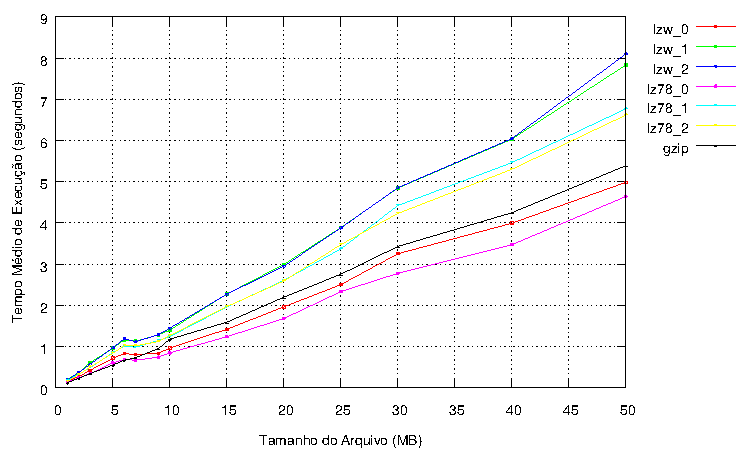
\includegraphics{images/natural_tempo_sem_lz77}
\caption{Tempo de compressão em função do tamanho do arquivo de entrada - sem o LZ77 para facilitar a visualização.}
\label{fig:e1}
\end{figure}

\begin{figure}
	{\centering Tempo Médio de Compressão - Teste 1 do LZ77\par}
	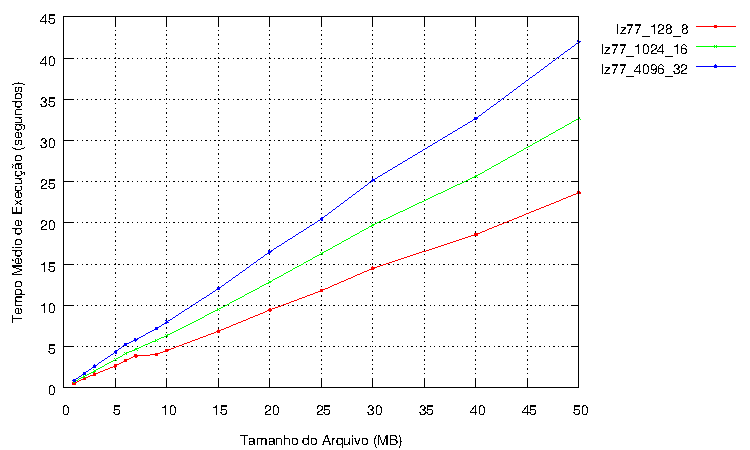
\includegraphics{images/natural_tempo_com_lz77}
\caption{Tempo de compressão em função do tamanho do arquivo de entrada - apenas o LZ77.}
\label{fig:e2}
\end{figure}

\begin{figure}
	{\centering Tamanho Médio dos Arquivos Comprimidos - Teste 1\par}
	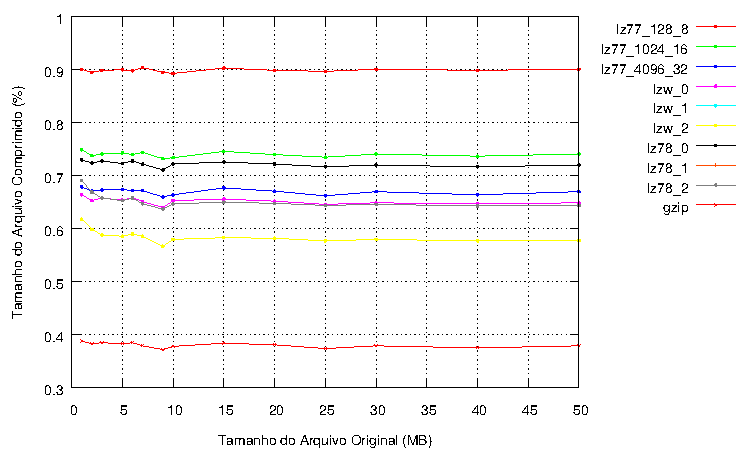
\includegraphics{images/natural_taxa}
\caption{Tamanho dos arquivos comprimidos em função dos tamanhos originais.}
\label{fig:e3}
\end{figure}

Separamos os tempos de execução do teste 1 nas figuras \ref{fig:e1} e \ref{fig:e2} apenas para facilitar a visualização. Note que os tempos do algoritmo LZ77 foram bem superiores aos demais em todas as suas configurações testadas. Os níveis 1 e 2 de compressão dos algoritmos LZ78 e LZW não causaram grande diferença nos tempos de execução. Todos os algoritmos e também a ferramenta \textit{gzip} apresentaram um crescimento linear do tempo de execução.

Como mostra a \figref{fig:e3}, todos os algoritmos apresentaram um comportamento aproximadamente constante em relação ao tamanho do arquivo comprimido. Note que os níveis 1 e 2 de compressão, tanto do LZ78 quanto do LZW, tiveram resultados indistinguíveis neste teste. A ferramenta \textit{gzip} se mostrou bastante superior em relação à taxa de compressão neste primeiro cenário.

Ainda no mesmo cenário de teste, medimos o tempo médio necessário para descomprimir os arquivos gerados. Como mencionamos, cada tamanho é representado por 3 arquivos distintos. Por isso, o tempo de descompressão é calculado como a média para descomprimir os 3 arquivos gerados na etapa anterior (de compressão). Apresentamos os resultados no gráfico da \figref{fig:e4}.

\begin{figure}
	{\centering Tempo Médio de Descompressão - Teste 1\par}
	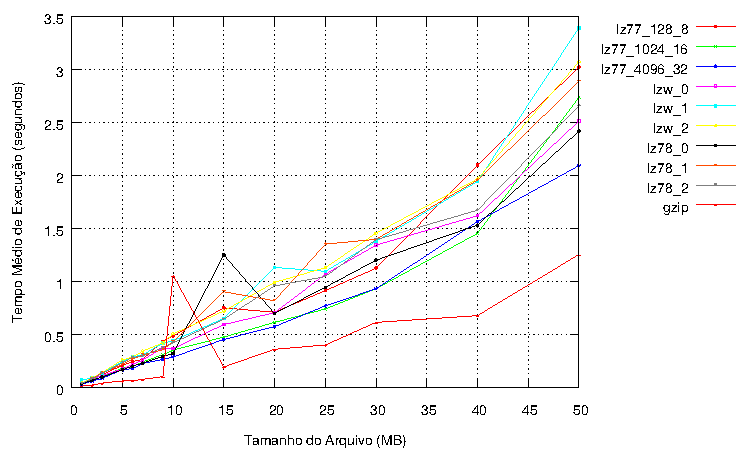
\includegraphics{images/natural_descompressao}
\caption{Tempo de descompressão em função do tamanho dos arquivos originais.}
\label{fig:e4}
\end{figure}

Em relação à descompressão, os algoritmos apresentaram um crescimento do tempo de execução aproximadamente linear. Algumas anomalias podem ser notadas na \figref{fig:e4}, provavelmente decorrentes de alguma característica particular dos arquivos utilizados. Os tempos de execução de todos os algoritmos são compatíveis, com exceção do \textit{gzip}, que cresce mais devagar. Em particular, o LZ77 consegue bons tempos de execução.

Embora os arquivos de texto nos ajudem a ter uma ideia do comportamento dos algoritmos, os tipos de arquivos que iremos comprimir são binários. Não podemos dizer, a princípio, o quão diferentes eles são dos arquivos de texto, principalmente porque não sabemos o quão redundante eles são e nem como as possíveis repetições presentes neles estão distribuídas. Por essa razão criamos um segundo cenário de testes no qual os arquivos apresentados aos algoritmos são pedaços de arquivos de índices gerados por nossas implementações do \textit{array} de sufixo e da árvore de sufixo. 

Utilizamos a mesma estratégia para a geração dos arquivos de teste: separamos os arquivos por tamanho de modo que cada tamanho fosse representado por 3 arquivos. Nossa escolha dos tamanhos, no entanto, foi um pouco diferente. Notamos que os arquivos de índice gerados, os que de fato serão comprimidos, têm, em geral, tamanho bem superior ao dos arquivos de texto original. Por isso, neste cenário de arquivos binários, utilizamos tamanhos maiores. Reportamos os resultados nos gráficos das figuras \ref{fig:e5}, \ref{fig:e6} e \ref{fig:e7}.

\begin{figure}
	{\centering Tempo Médio de Compressão - Teste 2 sem o LZ77\par}
	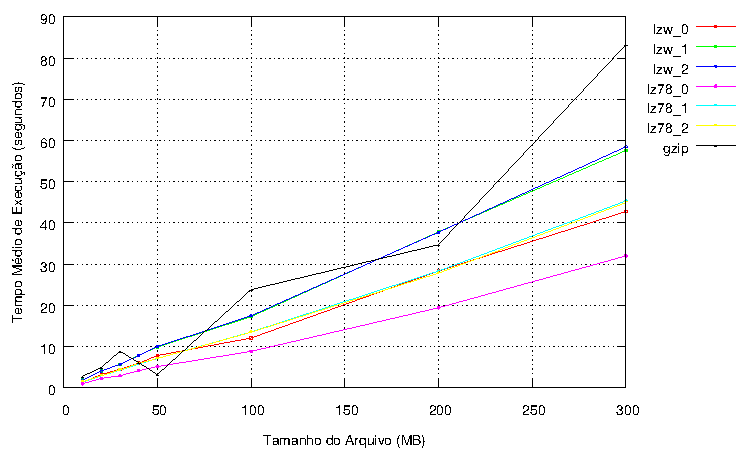
\includegraphics{images/binario_tempo_sem_lz77}
\caption{Tempo de compressão em função do tamanho do arquivo de entrada - sem o LZ77 para facilitar a visualização.}
\label{fig:e5}
\end{figure}

\begin{figure}
	{\centering Tempo Médio de Compressão - Teste 2 do LZ77\par}
	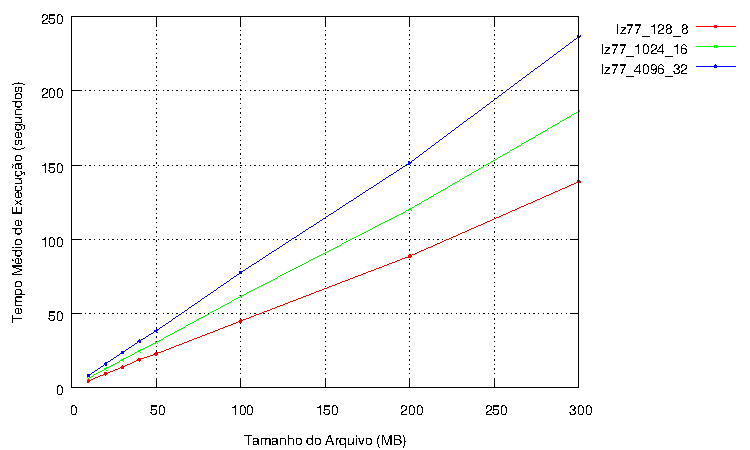
\includegraphics{images/binario_tempo_com_lz77}
\caption{Tempo de compressão em função do tamanho do arquivo de entrada - apenas o LZ77.}
\label{fig:e6}
\end{figure}

\begin{figure}
	{\centering Tamanho Médio dos Arquivos Comprimidos - Teste 2\par}
	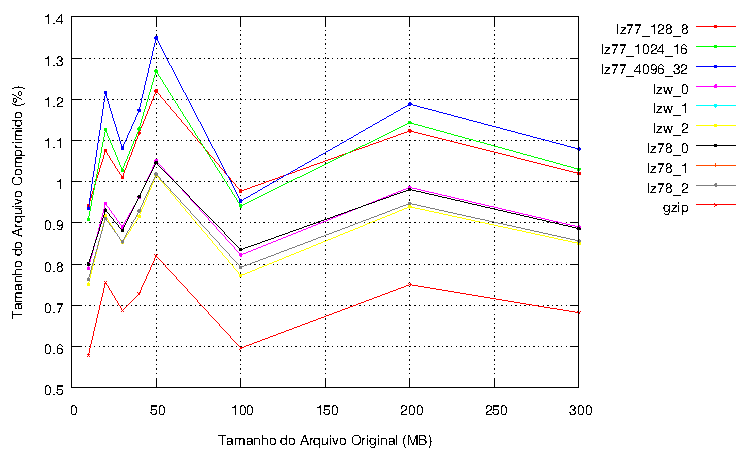
\includegraphics{images/binario_taxa}
\caption{Tamanho dos arquivos comprimidos em função dos tamanhos originais.}
\label{fig:e7}
\end{figure}


Os tempos médios de execução reportados nas figuras \ref{fig:e5} e \ref{fig:e6} não chegam a trazer grandes novidades em relação aos testes anteriores. Constatamos mais uma vez que esses tempos crescem linearmente com o tamanho dos arquivos.

A novidade fica por conta do tamanho dos arquivos comprimidos, mostradas no gráfico da \figref{fig:e7}. Alguns arquivos foram ``expandidos'' por alguns algoritmos. Em particular, o LZ77 com 4096 \textit{bytes} de \textit{buffer} e 32 de \textit{lookahead} chegou a aumentar um arquivo de 50MB em 30\%. É interessante também notar que a taxa de compressão não se comportou de maneira constante, como no teste anterior. Em parte isso se deve pela natureza dos arquivos de índice. Isso porque eles contém tanto o texto original quanto a estrutura de dados serializada. Por essa razão, alguns dos arquivos de testes, que foram extraídos aleatoriamente de arquivos de índice, tiveram maior quantidade de texto que outros.

Ressaltamos que também o \textit{gzip} experimentou uma diminuição na sua taxa de compressão quando apresentado aos arquivos binários. Enquanto que no cenário anterior ele reduzia os arquivos a 40\% de seu tamanho original, agora ele gera arquivos com cerca de 70\% de seu tamanho original. Esse fato atesta que os arquivos binários apresentados são mais ``desafiadores'' para os algoritmos de compressão.

Por fim reportamos na \figref{fig:e8} os tempos de descompressão dos arquivos binários comprimidos. Podemos perceber que o \textit{gzip} possui um tempo de execução bastante inferior aos das nossas implementações. 


\begin{figure}
	{\centering Tempo Médio para Descompressão do Teste 2\par}
	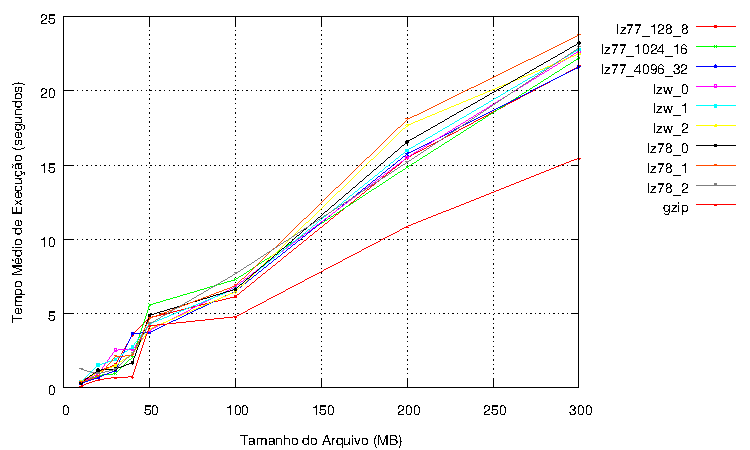
\includegraphics{images/binario_descompressao}
\caption{Tempo de descompressão em função do tamanho dos arquivos originais.}
\label{fig:e8}
\end{figure}


\subsection{Construção dos Índices}

Os próximos testes que apresentaremos tentam medir a eficiência da construção de cada índice. Neles, apresentamos arquivos de diferentes tamanhos para cada implementação de índice. Esperamos tanto medir o tempo necessário para a construção dos índices, sem levar em conta os tempos de compressão nem de salvamento em disco, quanto descobrir o tamanho máximo de texto de entrada suportado pelas nossas implementações. Além do tempo de construção, medimos também o tamanho do arquivo de índice \textit{descomprimido}. Esse tamanho serve para indicar o crescimento no uso de memória \textit{RAM} de cada índice. Além disso ele também está diretamente ligado ao tempo que a etapa de compressão levará.

Utilizamos arquivos de texto em inglês separados por tamanho. Cada tamanho foi representado por 3 arquivos diferentes. Cada aquivo, por sua vez, foi apresentando 3 vezes a cada índice. Calculamos o tempo de criação de cada índice como a média do tempo das 9 execuções. O tamanho do arquivo de índice gerado foi calculado como a média dos 3 arquivos distintos gerados. Apresentamos os resultados nos gráficos das figuras \ref{fig:e9} e \ref{fig:e10} a seguir.

\begin{figure}
	{\centering Tempo Médio para Criação dos Índices\par}
	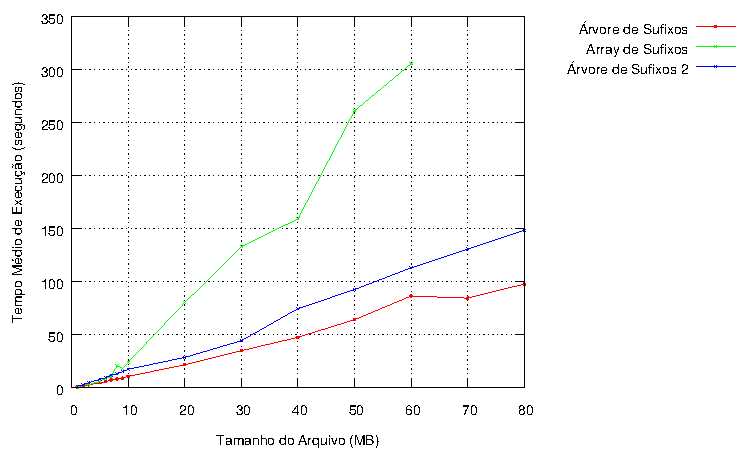
\includegraphics{images/index_criacao}
\caption{Tempo de criação dos índices em função do tamanho dos arquivos de entrada.}
\label{fig:e9}
\end{figure}

\begin{figure}
	{\centering Tamanho Médio do Arquivo de Índice Descomprimido\par}
	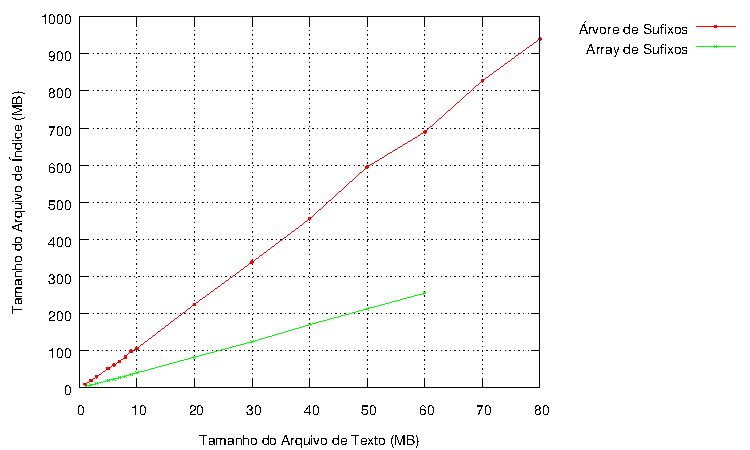
\includegraphics{images/index_tamanho}
\caption{Tamanho do arquivo descomprimido de índice em função do tamanho dos arquivos de entrada.}
\label{fig:e10}
\end{figure}


Nas figuras \ref{fig:e9} e \ref{fig:e10} verificamos que tanto o tempo de construção como o tamanho do arquivo gerado pela árvore de sufixos cresce linearmente com o tamanho da entrada, como era esperado. Notamos que a implementação alternativa, que chamamos de árvore de sufixos 2, tem um tempo de construção um pouco maior. Não a incluímos no gráficos dos tamanhos dos arquivos porque ela produz exatamente o mesmo arquivo que a implementação ``tradicional''.

Já o \textit{array} de sufixos apresenta um tempo de criação superior, especialmente para entradas maiores. Isso também era esperado já que a complexidade de sua construção é maior. Por outro lado, os arquivos gerados crescem linearmente com o tamanho da entrada. Naturalmente isso já era esperado, uma vez que neles são armazenados dois vetores com tamanho proporcional ao da entrada. Outro resultado que não chega a surpreender é o fato desses arquivos serem significativamente menores que os gerados pela árvore de sufixos.


Ressaltamos que o gráfico da \figref{fig:e10} reflete, de certa forma, o crescimento do uso da memória \textit{RAM} para a criação dos índices. No entanto, esses arquivos guardam apenas o essencial para que as estruturas sejam reconstruídas de maneira eficiente. Por essa razão, as estruturas que eles armazenam, quando completas, consomem uma quantidade de memória consideravelmente maior que o tamanho dos arquivos onde estão armazenadas. Por exemplo, a árvore de sufixos para uma entrada de 80MB chega a consumir quase 3GB de memória \textit{RAM}, embora seja armazenada em um arquivo de pouco mais de 900MB.

Deixamos de executar os testes com o \textit{array} de sufixos a partir da entrada de 60MB por conta do elevado tempo de execução. 

\subsection{Buscas}

Testamos nossa ferramenta com o objetivo de medir a eficiência das buscas com os dois índices que foram implementados. Para isso, geramos arquivos de textos em inglês de tamanhos diferentes e arquivos de padrões, também em inglês com tamanho igual aos arquivos de texto. Para a realização dos testes utilizamos a opção de apenas contar a quantidade de ocorrências. Naturalmente que o tempo de execução da ferramenta quando imprime as linhas das ocorrências é maior.

Executamos a ferramenta \textit{grep} como forma de comparar os tempos de execução de estratégias de buscas diferentes, isto é, a busca sem indexação e a com indexação. O comando utilizado para invocar essa ferramenta foi \textit{grep -F -e padrao aquivo\_de\_texto -c}. A configuração \textit{-F} faz com que o \textit{grep} trate os padrões como cadeias fixas e não como expressões regulares. Isso é importante porque os padrões podiam conter caracteres como ``*, [ ,]'' e outros que têm significado especial para expressões regulares. A configuração \textit{-c} faz o \textit{grep} contar somente as \textit{linhas} que contém alguma ocorrência. Note que esse não é exatamente o valor que queríamos obter, mas é a única opção que faz o \textit{grep} não imprimir cadeias\footnote{Também consideramos utilizar o \textit{grep} com a opção \textit{-o} e processar o resultado, como no primeiro projeto: \textit{grep -F -e padrao arquivo\_de\_texto -o $\vert$ wc -l}. Mas preferimos utilizar o \textit{grep} da maneira mais eficiente possível.}.

Para este teste, os arquivos de índices foram comprimidos com o algoritmo LZW. 

Para cada tipo de índice nós reportamos o \textit{tempo de carregamento}, que leva em conta a leitura e descompressão do arquivo de índice bem como qualquer outro processamento necessário para completar a estrutura de dados. Naturalmente que esse carregamento só precisa ser feito 1 única vez. O \textit{tempo de busca}, por sua vez, é a soma dos tempos de buscas de todos os padrões. Como mencionamos anteriormente, os arquivos de padrões tinham o mesmo tamanho dos arquivos de texto. Registramos os resultados na tabela \ref{tab:t2}.

\begin{table}
	\begin{tabular}{c|c|c|c|c|c}
		Tamanho do Texto & \multicolumn{2}{c|}{Árvore de Sufixos} & \multicolumn{2}{c|}{\textit{Array} de Sufixos} & \textit{grep} \\
						 & 		Carregamento & Busca			  &			 Carregamento & Busca				   & \\
		\hline
            1MB &  0.50s  &  0.10s &  0.23s &  0.16s & $>$2min \\
            2MB &  1.09s  &  0.26s &  0.46s &  0.48s & $>$2min \\
            3MB &  1.57s  &  0.31s &  0.79s &  0.68s & $>$2min \\
            4MB &  2.21s  &  0.41s &  1.13s &  0.81s & $>$2min \\
            5MB &  2.74s  &  0.14s &  0.98s &  1.02s & $>$2min \\
            6MB &  3.18s  &  0.57s &  1.64s &  1.53s & $>$2min \\
            7MB &  3.59s  &  0.70s &  1.67s &  1.57s & $>$2min \\
            8MB &  4.47s  &  0.55s &  1.82s &  2.04s & $>$2min \\
            9MB &  4.92s  &  0.99s &  2.11s &  2.33s & $>$2min \\
           10MB &  4.94s  &  0.54s &  2.14s &  1.92s & $>$2min \\
           20MB & 10.17s  &  1.28s &  4.46s &  4.37s & $>$2min \\
           50MB & 25.79s  &  5.61s & 11.61s & 12.05s & $>$2min \\
           60MB & 34.76s  &  7.79s & 14.31s & 15.86s & $>$2min \\
           70MB & 43.69s  &  8.40s & 17.00s & 17.56s & $>$2min \\
	\end{tabular}
\caption{O tempo da busca por padrões usando os diferentes índices e a ferramenta \textit{grep}. Os arquivos de padrões têm o mesmo tamanho dos arquivos de entrada.}
\label{tab:t2}
\end{table}

Notamos, pela tabela \ref{tab:t2} que a árvore de sufixos é mais eficiente na busca mesmo para arquivos pequenos. Por outro lado, ela possui um tempo de carregamento maior. No entanto, a depender da aplicação, esse tempo de carregamento é compensado pela rapidez das buscas.

A ferramenta \textit{grep} apresentou um desempenho muito ruim neste primeiro teste, superando bastante os tempos de carregamento e buscas. No entanto, reconhecemos que esse resultado foi influenciado pela maneira de criação dos arquivos de teste. Isso porque não somente o tamanho dos padrões e do texto afetam o tempo total do \textit{grep}, mas também a \textit{quantidade de consultas} realizadas. Essa variável, no entanto, não foi controlada e, por essa razão, mesmo o menor arquivo de teste continha mais de 100000 consultas. Esse é, naturalmente, um cenário válido e mostra como a indexação é uma boa estratégia para suportar uma grande quantidade de consultas a um mesmo texto. No entanto, esses resultados nos motivaram a criar um segundo cenário de teste, no qual os arquivos de padrões continham menos consultas. 

Conduzimos a segunda rodada de testes como a primeira, mas restringindo os arquivos de padrões a 100 linhas. Com isso esperamos conseguir executar o \textit{grep} em um tempo razoável. Os resultados são reportados na tabela \ref{tab:t3} a seguir.

\begin{table}
	\begin{tabular}{c|c|c|c|c|c}
		Tamanho do Texto & \multicolumn{2}{c|}{Árvore de Sufixos} & \multicolumn{2}{c|}{\textit{Array} de Sufixos} & \textit{grep} \\
						 & 		Carregamento & Busca			  &			 Carregamento & Busca				   & \\
		\hline
   1MB &  0.49s  & 0.04s &  0.19 & 0.02s &  0.72s  \\    
   2MB &  1.07s  & 0.05s &  0.43 & 0.03s &  1.30s  \\    
   3MB &  1.60s  & 0.15s &  0.66 & 0.02s &  1.49s  \\    
   4MB &  2.01s  & 0.05s &  0.93 & 0.04s &  2.00s  \\    
   5MB &  2.56s  & 0.15s &  1.10 & 0.07s &  3.03s  \\    
   6MB &  3.16s  & 0.02s &  1.33 & 0.04s &  4.53s  \\    
   7MB &  3.79s  & 0.06s &  1.44 & 0.07s &  3.80s  \\    
   8MB &  4.09s  & 0.01s &  1.72 & 0.13s &  3.86s  \\    
   9MB &  5.15s  & 0.14s &  1.82 & 0.03s &  4.53s  \\    
  10MB &  4.96s  & 0.02s &  2.23 & 0.00s &  3.06s  \\    
  20MB & 10.08s  & 0.01s &  4.31 & 0.11s &  9.71s  \\    
  50MB & 26.99s  & 0.33s & 11.26 & 0.11s & 28.55s  \\    
  60MB & 31.57s  & 0.22s & 13.25 & 0.18s & 21.80s  \\    
  70MB & 38.07s  & 0.80s & 15.79 & 0.15s & 19.39s  \\    
	\end{tabular}
\caption{O tempo da busca por padrões usando os diferentes índices e a ferramenta \textit{grep}. Os arquivos de padrões tem 100 linhas.}
\label{tab:t3}
\end{table}


Como vemos na tabela \ref{tab:t3}, o tempo de busca do \textit{grep} é sempre superior ao da nossa ferramenta. Isso já era esperado tanto pelo que vimos no teste anterior quanto pelo fato de que o \textit{grep} precisa processar todo o arquivo texto para cada padrão.

\section{Considerações Finais}

A implementação dos índices e dos algoritmos de compressão foi bastante desafiadora pois toda decisão (boa ou má) tinha grande impacto na escalabilidade da ferramenta. Os índices exigem muito cuidado no uso da memória, pois tendem a se tornar estruturas muito grandes. Por outro lado, os algoritmos de compressão precisam ser rápidos, uma vez que recebem essas mesmas estruturas como entrada.

Com os testes que executamos, pudemos verificar, principalmente em relação à árvore de sufixos, que a memória é o gargalo dos índices e não o tempo de criação propriamente. Já em relação aos algoritmos de compressão e descompressão, verificamos que o tempo de compressão e a taxa de compressão são variáveis de grande impacto na eficiência geral da ferramenta. Em particular, em algumas situações pudemos observar que os arquivos binários de índice, após passarem por um demorado processo de compressão, eram na verdade ``expandidos''. Pelos testes que fizemos, pudemos concluir que isso se deve principalmente à natureza dos próprios arquivos de índice.

Por fim, pudemos concluir, na prática, que a estratégia de construção de índice é bastante vantajosa quando se pretende fazer várias consultas em um mesmo texto. Isso segue diretamente dos testes que realizamos com a ferramenta \textit{grep}, a qual é bastante eficiente.




\end{document}
